\documentclass[a4paper,11pt,spanish,sans]{exam}
\usepackage[spanish]{babel}
%\usepackage[utf8]{inputenc}
\usepackage{multicol}
%\usepackage[latin1]{inputenc}
\usepackage{fontspec}%la posta para las tildes con lualatex
\usepackage[margin=0.5in]{geometry}
\usepackage{amsmath,amssymb}
\usepackage{multicol}
\usepackage{natbib}
\usepackage{graphicx}
\usepackage{hyperref}
\usepackage{epstopdf}
\usepackage{capt-of}
\usepackage{gensymb}
\usepackage{float}
\usepackage{wrapfig}
\usepackage{pst-fractal}
%\usepackage{animate}
\usepackage[usenames]{color}
%para graficos
\usepackage{pgf,tikz}
\usepackage{mathrsfs}
\usetikzlibrary{arrows}
\usepackage{pst-fractal}
\usetikzlibrary{decorations.markings}
\usetikzlibrary{shapes.geometric}
\usetikzlibrary{shapes,snakes}
\usepackage{tkz-euclide}
\usetkzobj{all}

\newcommand{\class}{Matemática: Integradora de 4to }
\newcommand{\term}{Diciembre 2015}
\newcommand{\examnumuno}{Tema 1}
\newcommand{\examnumdos}{Tema 2}
\newcommand{\examnumvulcano}{Tema 3}
\newcommand{\examprof}{Alexis Gomel}
\newcommand{\examdate}{20/11/2015}
\newcommand{\timelimit}{60 Minutes}%no lo uso
\newcommand{\Ts}{\rule{0pt}{2.8ex}}       % Top strut
\newcommand{\Bs}{\rule[-1.5ex]{0pt}{0pt}} % Bottom strut
%el header de las hojas.
\pagestyle{head}
\firstpageheader{}{}{}
%\runningheader{\class}{\examnumuno\ - pagina \thepage\ de \numpages}{\examdate}
%\runningheadrule

\begin{document}
	\noindent 
	\begin{minipage}{0.92\linewidth}
		\begin{tabular*}{\textwidth}{l @{\extracolsep{\fill}} r @{\extracolsep{6pt}} l}
			\textbf{\class} & \textbf{Profesor: \examprof}\\
			\textbf{\examnumuno}  & \textbf{}   \\
			%& Teaching Assistant & %VII la venganza de adrian  \makebox[2in]{\hrulefill}
			\textbf{Nombre: } \makebox[2in]{\hrulefill} & \textbf{\examdate} 
		\end{tabular*}\\
	\end{minipage}
	\begin{minipage}[r]{0.08\linewidth}
		\begin{flushright}
			
\includegraphics[width=\linewidth]{bost.png}
		\end{flushright}
	\end{minipage}\\
	\rule[2ex]{\textwidth}{2pt}

\begin{center}
	\textsl{\textbf{\underline{Justificar}}} cada respuesta. La evaluación se entrega \textbf{\underline{escrita en tinta}}.\\
	Si se traban con un ejercicio sigan con el siguiente.
	May the force be with you.
\end{center}
\begin{table}[h]
	\centering
	%\caption{My caption}
	\label{my-label}
	\begin{tabular}{|l|c|c|c|c|c|c|c|c|c|}
		\hline
		Ejercicio        & 1 & 2 & 3 & 4 & 5 & 6 & 7 & Nota & Hojas \\ \hline
		Puntaje máximo   & 0,5 & 0,5 & 2 & 2 & 2 & 1,5 & 1,5 & 10 &  Entregadas \\ \hline
		Puntaje obtenido &   &   & & & & & &  &   \\ \hline
	\end{tabular}
\end{table}

\begin{enumerate}
	
\item \section*{Numeros Reales y conjuntos (0,5 puntos) }
Graficar los conjuntos $\mathbb{N}$, $\mathbb{R}$, $\mathbb{Q}$, $\mathbb{C}$, $\mathbb{I}$, $\mathbb{Z}$, $\mathbb{I}m$ (imaginarios) como diagramas de Venn.

\item  \section*{Radicacion (0,5 puntos)}

\begin{enumerate}
	\item $\dfrac{\sqrt{5}-2}{2+\sqrt{5}}$
	\item $\dfrac{10}{2\sqrt{5}+5\sqrt{2}}$
\end{enumerate}

\item  \section*{Cuadraticas (2 puntos)}
\begin{enumerate}
	\item Bicuadratica: $x^4-10x^2+9=0$
	\item Graficar la siguiente función y expresarla en sus tres formas (normal, canónica y factorizada).
	
	$y=2(x+1)^2-3 $
\end{enumerate}

\item  \section*{Logaritmos y exponenciales (2 puntos)}
\begin{enumerate}
	
	\item $3.\log_2(x)-2.\log_4(x^2)=2$
	
	\item Encontar el valor de x para que $2^x+2^{x+1}+\dfrac{5}{4}2^{x+2}=256$
	
\end{enumerate}

\item  \section*{Trigonometria (1,5 puntos)}
%\item Resolver los siguientes triángulos rectángulos. (Calcular los lados, los ángulos y sus razones trigonométricas). \label{rectangulos}\\

%	\begin{minipage}{0.45\linewidth}
%		
%		\begin{tikzpicture}[thick]
%		\coordinate (O) at (0,0);
%		\coordinate (A) at (3.5,0);
%		\coordinate (B) at (0,2.6);
%		\draw (O)--(A)--(B)--cycle;
%		
%		\tkzLabelSegment[below=2pt](O,A){$b$}
%		\tkzLabelSegment[left=2pt](O,B){$a$}
%		\tkzLabelSegment[above right=2pt](A,B){$h$}
%		
%		\tkzMarkRightAngle[fill=orange,size=0.6,opacity=.4](A,O,B)% square angle here
%		\tkzLabelAngle[pos = 0.35](A,O,B){$\hat{\gamma}$}
%		
%		\tkzMarkAngle[fill= orange,size=0.8cm,%
%		opacity=.4](B,A,O)
%		\tkzLabelAngle[pos = 0.6](B,A,O){$\hat{\alpha}$}
%		
%		\tkzMarkAngle[fill= orange,size=0.8cm,%
%		opacity=.4](O,B,A)
%		\tkzLabelAngle[pos = 0.5](O,B,A){$\hat{\beta}$}
%		
%		\end{tikzpicture}
%		
%	\end{minipage}
%	\begin{minipage}{0.55\linewidth}
%		\begin{enumerate}
%			%\item $a=3km$,  $\quad b=4km$ .	Expresar los resultados de los ángulos en el sistema sexagesimal.
%			%\item $a=2cm$, $\quad b=1cm$
%			\item $a=30km$,  $\quad b=20km$ .	Expresar los resultados de los ángulos en el sistema sexagesimal.
%			%\item $a=5cm$, $\quad \sin(\beta)=\frac{1}{\sqrt{2}}$. Expresar los resultados de los ángulos en Radianes.
%			%\item $a=5cm$, $\quad \cos(\alpha)=\frac{\sqrt{2}}{2}$
%			\item $a=5cm$, $\quad \cos(\alpha)=\frac{\sqrt{3}}{2}$ 
%		\end{enumerate}
%	\end{minipage}
Encontrar el lado restante y los ángulos internos.

\begin{tikzpicture}[thick]
\coordinate (O) at (0,0);
\coordinate (A) at (3,0);
\coordinate (B) at (2.5,1.5);
\draw (O)--(A)--(B)--cycle;

\tkzLabelSegment[below=2pt](O,A){$10m$}
\tkzLabelSegment[left=2pt](O,B){$15m$}
\tkzLabelSegment[above right=2pt](A,B){}

\tkzMarkAngle[fill=orange,size=0.3cm,opacity=.4](A,O,B)
\tkzLabelAngle[pos = -0.7](A,O,B){$\hat{\gamma}=30\degree $}

\tkzMarkAngle[fill= orange,size=0.3cm,%
opacity=.4](B,A,O)
\tkzLabelAngle[ pos= -0.4 ](B,A,O){$\hat{\alpha}$}

\tkzMarkAngle[fill= orange,size=0.3cm,%
opacity=.4](O,B,A)
\tkzLabelAngle[pos = -0.4](O,B,A){$\hat{\beta}$}
\end{tikzpicture}

\item  \section*{Complejos (1,5 puntos)}

\begin{enumerate}
	\item Resolver la siguiente ecuación y graficar el resultado en el plano complejo.
	
	$-z(4+iz)+1=(4+2i)z+i^4$

\end{enumerate}
	
\item \section*{Funciones Racionales (2 puntos)}

	\begin{minipage}{0.5\textwidth}
		\centering
		%\begin{table}[!h]
		%\caption{mc1}
		\label{mc1}
		\begin{tabular}{|c|c|c|}
			\hline
			$\dfrac{x^2}{(x-1)^3}$  & $\dfrac{x^3}{(x-1)^2}$ & $\dfrac{x^3}{(x+1)^2}$ \Ts \Bs   \\ \hline
			&   &      \\ \hline
		\end{tabular}\\
		%\end{table}
		%\begin{figure}[h]
		\centering
		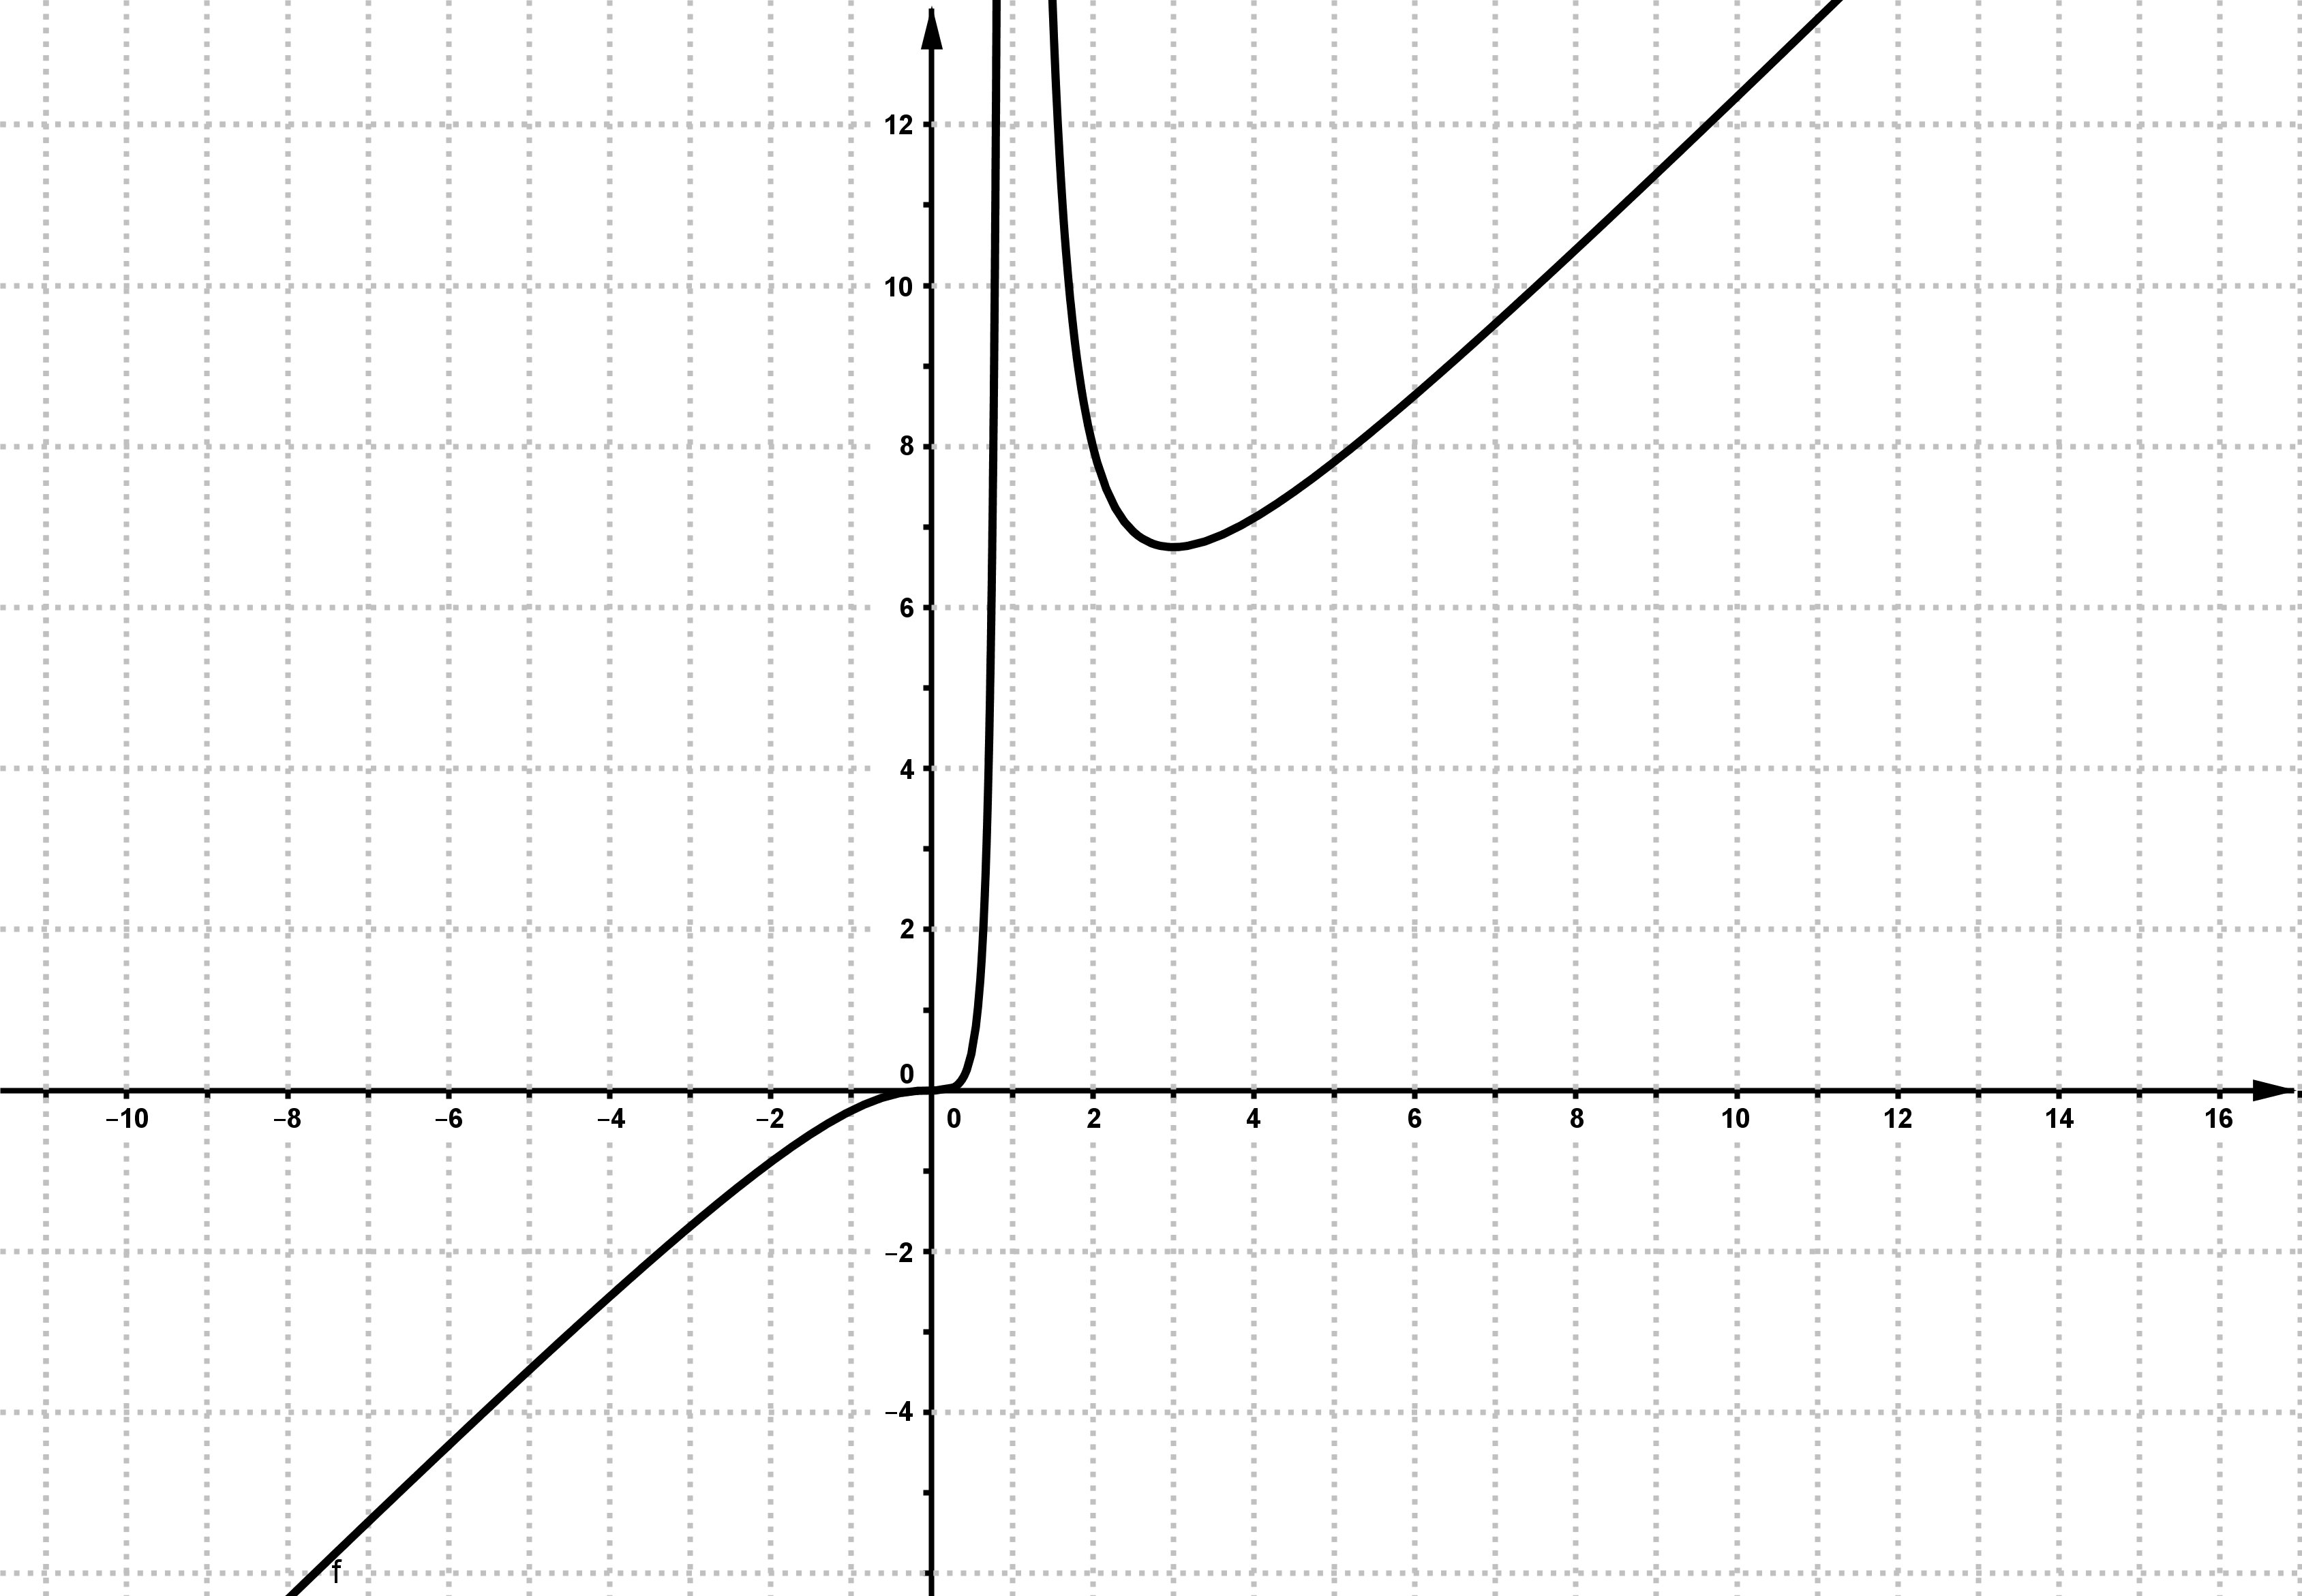
\includegraphics[width= 0.95\linewidth]{integradora1.png}
		%\end{figure}
		%graficos
	\end{minipage}
	\begin{minipage}{.5\textwidth}
		\centering
		%\begin{table}[!h]
		%\caption{mc1}
		%\label{mc1}
		\begin{tabular}{|c|c|c|}
			\hline
			$\dfrac{5x^2}{(x-2)(x+2)}$  & $\dfrac{x^2}{5(x-2)(x+2)}$ & $\dfrac{5(x-2)(x+2)}{x^3}$ \Ts \Bs   \\ \hline
			&   &      \\ \hline
		\end{tabular}\\
		%\end{table}
		%\begin{figure}[h]
		\centering
		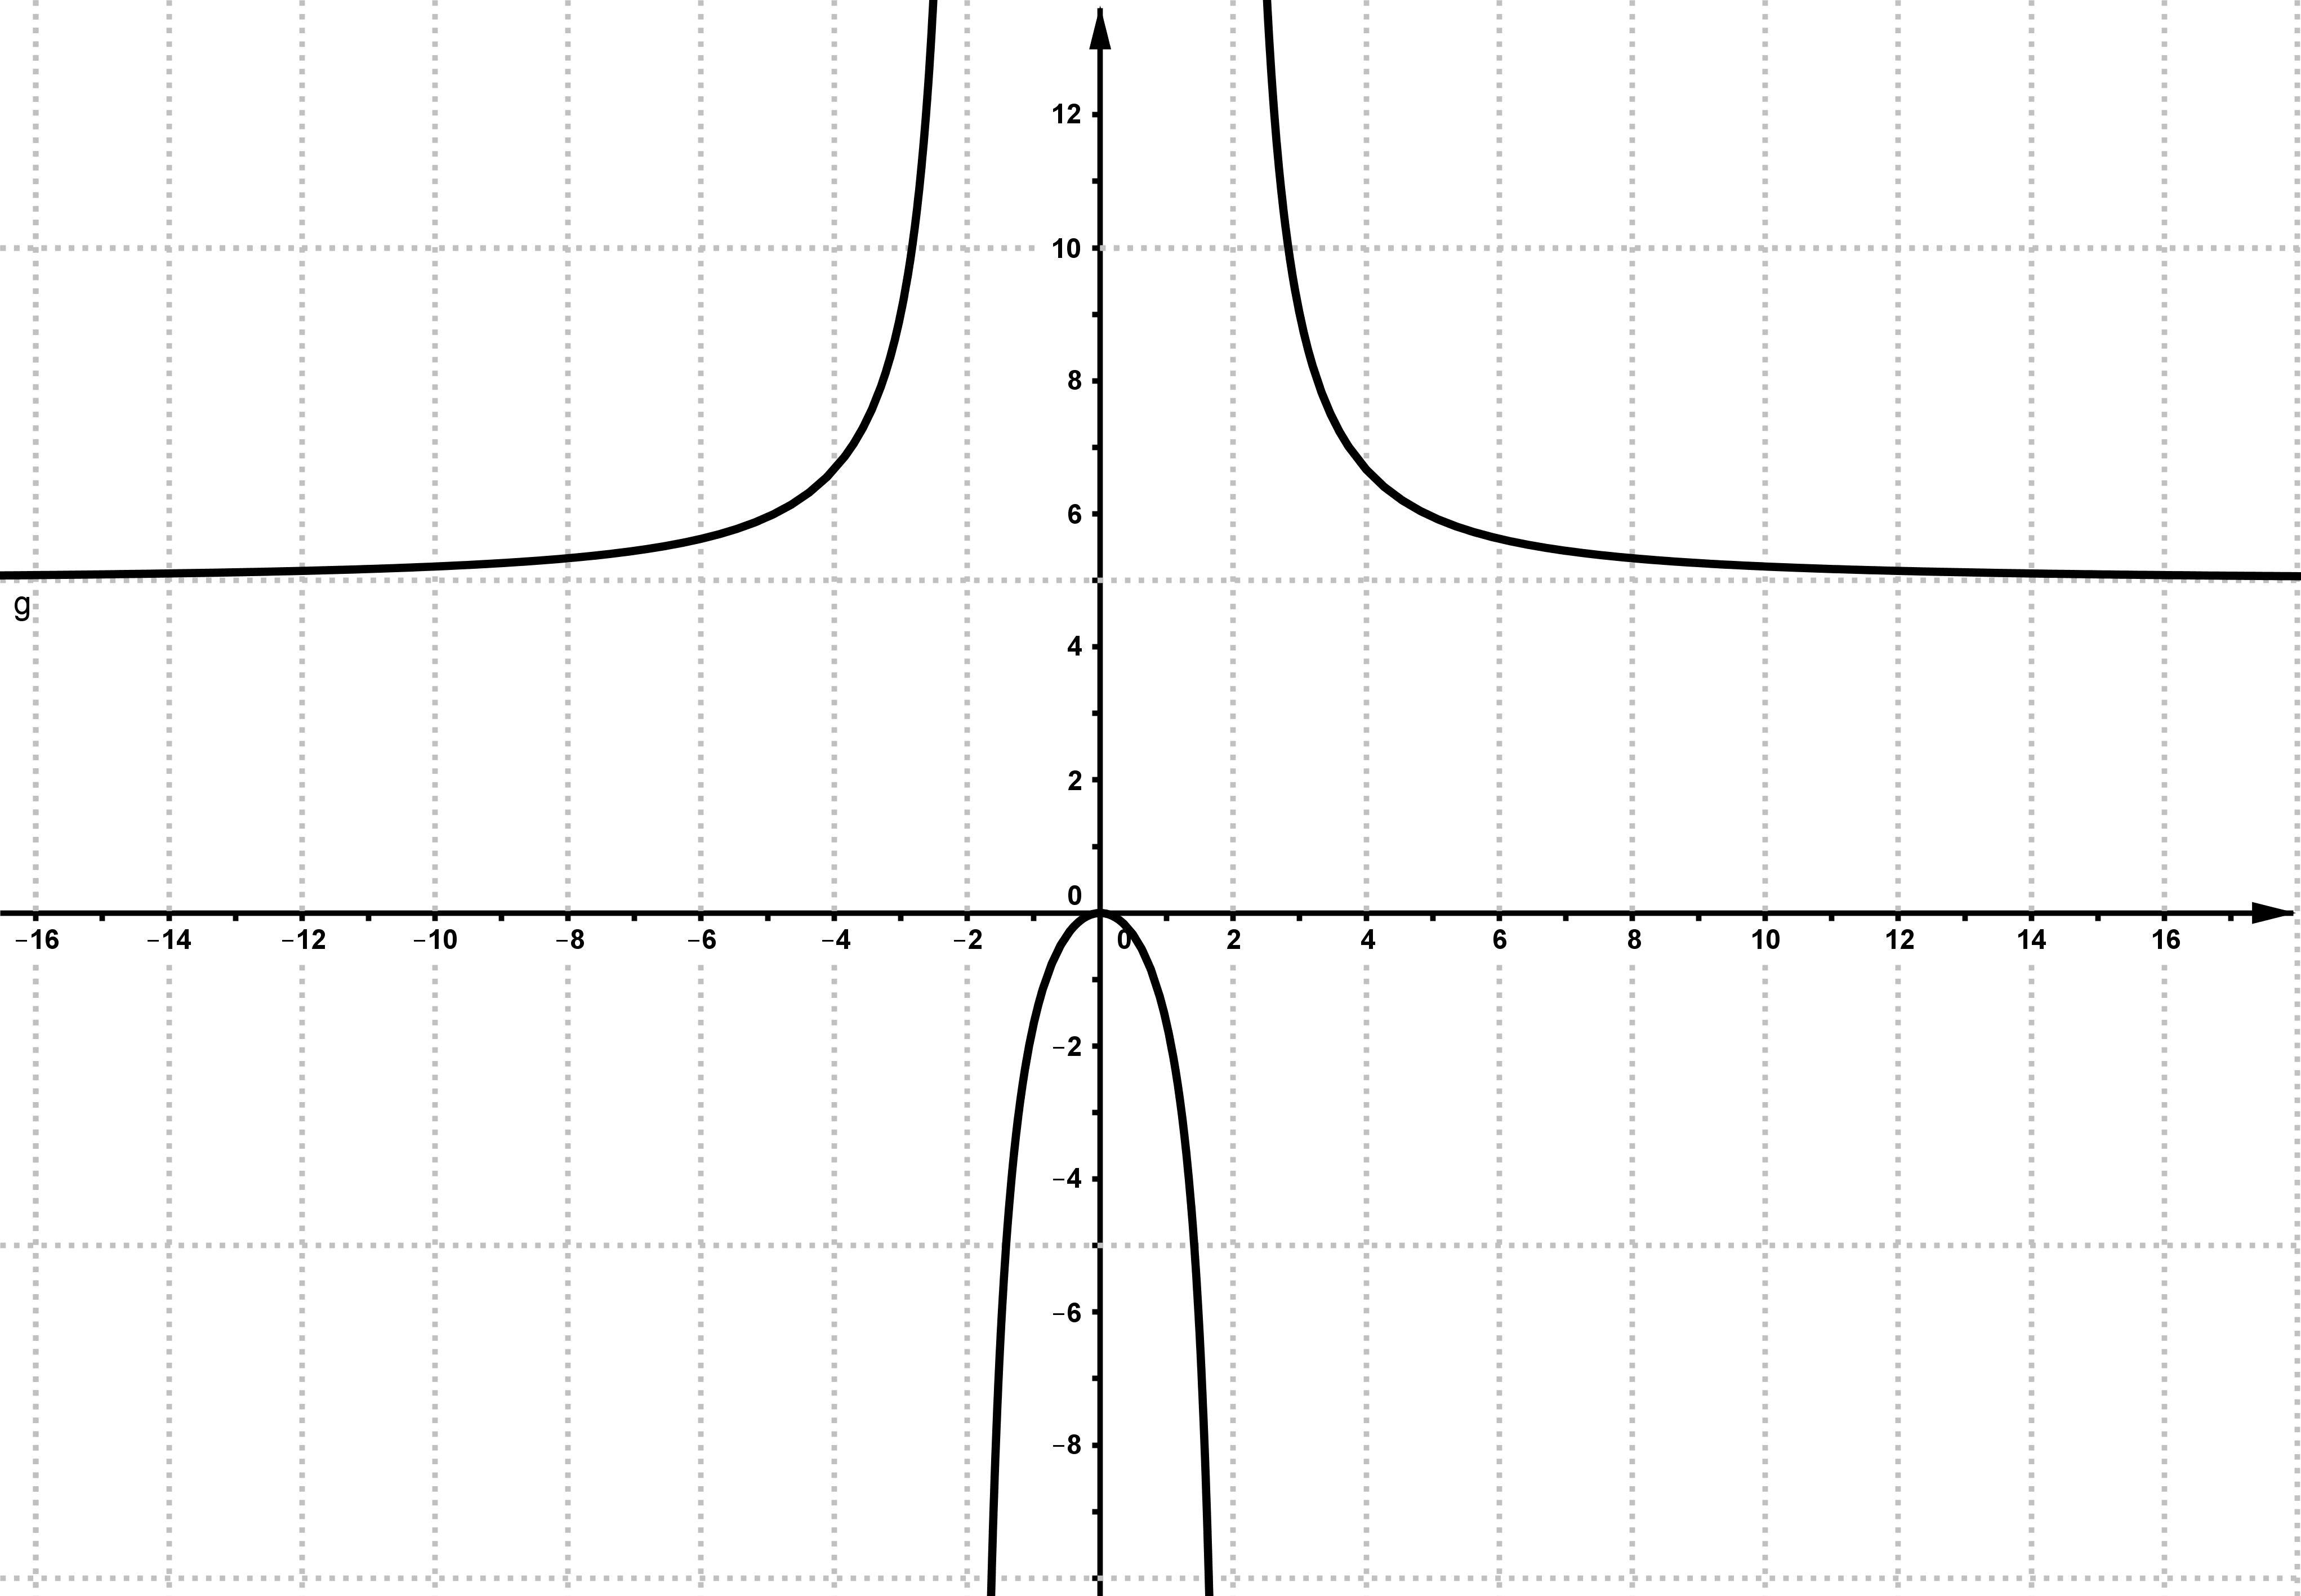
\includegraphics[width= 0.95\linewidth]{integradora2.png}
		%\end{figure}
	\end{minipage}\\
	              
	
	2. Encontrar todos los valores de $x$ tal que: $\dfrac{3x-1}{x+1}<3$
	\\



\end{enumerate}\\

\textbf{\underline{Hoja de formulas}:} . \\

\begin{minipage}{0.5\linewidth}
	
	\begin{tikzpicture}[thick]
	\coordinate (O) at (0,0);
	\coordinate (A) at (3.5,0);
	\coordinate (B) at (-1,3);
	\draw (O)--(A)--(B)--cycle;
	
	\node at (O) [below left=2pt]{$a$};
	\node at (A) [right=2pt]{$b$};
	\node at (B) [above left=2pt]{$c$};
	
	\tkzLabelSegment[below=2pt](O,A){}
	\tkzLabelSegment[left=2pt](O,B){}
	\tkzLabelSegment[above right=2pt](A,B){}
	
	\tkzMarkAngle[fill=orange,size=0.6,opacity=.4](A,O,B)% square angle here
	\tkzLabelAngle[pos = 0.35](A,O,B){$\hat{a}$}
	
	\tkzMarkAngle[fill= orange,size=0.8cm,%
	opacity=.4](B,A,O)
	\tkzLabelAngle[pos = 0.6](B,A,O){$\hat{b}$}
	
	\tkzMarkAngle[fill= orange,size=0.7cm,%
	opacity=.4](O,B,A)
	\tkzLabelAngle[pos = 0.5](O,B,A){$\hat{c}$}
	\end{tikzpicture}
	
\end{minipage}
\begin{minipage}{0.5\linewidth}
	\textbf{Teorema del seno}:
	
	\[
	\frac{\overline{ab}}{\sin(\hat{c})}=\frac{\overline{ac}}{\sin(\hat{b})}=\frac{\overline{bc}}{\sin(\hat{a})}
	\]
	
	
	\textbf{Teorema del coseno}:
	
	\[
	\overline{ab}^2=\overline{ac}^2 + \overline{bc}^2 - 2.\overline{bc}.\overline{ac}.\cos(\hat{c})
	\]
\end{minipage}

Pitagoras: $
(cat.op)^2+(cat.ady)^2=h^2
$

Cuadráticas:

$y=ax^2+bx+c$

$y=a(x-x_v)^2+y_v$

$y=a(x-x_1)(x-x_2)$

$x_v=\frac{-b}{2a}$

Cambio de base: $\log_a(b)=\dfrac{\log_c(b)}{\log_c(a)}$

\rule[2ex]{\textwidth}{1pt}

“Eppur si muove” (y sin embargo se mueve..)  -Galileo Galilei 

\newpage

	\noindent 
	\begin{minipage}{0.92\linewidth}
		\begin{tabular*}{\textwidth}{l @{\extracolsep{\fill}} r @{\extracolsep{6pt}} l}
			\textbf{\class} & \textbf{Profesor: \examprof}\\
			\textbf{\examnumdos}  & \textbf{}   \\
			%& Teaching Assistant & %VII la venganza de adrian  \makebox[2in]{\hrulefill}
			\textbf{Nombre: } \makebox[2in]{\hrulefill} & \textbf{\examdate} 
		\end{tabular*}\\
	\end{minipage}
	\begin{minipage}[r]{0.08\linewidth}
		\begin{flushright}
			
\includegraphics[width=\linewidth]{bost.png}
		\end{flushright}
	\end{minipage}\\
	\rule[2ex]{\textwidth}{2pt}

\begin{center}
	\textsl{\textbf{\underline{Justificar}}} cada respuesta. La evaluación se entrega \textbf{\underline{escrita en tinta}}.\\
	Si se traban con un ejercicio sigan con el siguiente.
	May the force be with you.
\end{center}
\begin{table}[h]
	\centering
	%\caption{My caption}
	\label{my-label}
	\begin{tabular}{|l|c|c|c|c|c|c|c|c|c|}
		\hline
		Ejercicio        & 1 & 2 & 3 & 4 & 5 & 6 & 7 & Nota & Hojas \\ \hline
		Puntaje máximo   & 0,5 & 0,5 & 2 & 2 & 2 & 1,5 & 1,5 & 10 &  Entregadas \\ \hline
		Puntaje obtenido &   &   & & & & & &  &   \\ \hline
	\end{tabular}
\end{table}


\section{Numeros Reales y conjuntos (0,5 puntos) }
Graficar los conjuntos $\mathbb{N}$, $\mathbb{R}$, $\mathbb{Q}$, $\mathbb{C}$, $\mathbb{I}$, $\mathbb{Z}$, $\mathbb{I}m$ (imaginarios) como diagramas de Venn.

\section{Radicacion (0,5 puntos)}

\begin{enumerate}
	\item $\dfrac{\sqrt{7}-3}{3+\sqrt{7}}$
	\item $\dfrac{21}{3\sqrt{7}+7\sqrt{3}}$
\end{enumerate}

\section{Cuadraticas (2 puntos)}
\begin{enumerate}
	\item Bicuadratica: $x^4-13x^2+36=0$
	\item Graficar la siguiente función y expresarla en sus tres formas (normal, canónica y factorizada).
	
	$y=2(x-3)^2-5 $
\end{enumerate}

\section{Logaritmos y exponenciales (2 puntos)}
\begin{enumerate}
	
	\item $-\log_9(x^2)+4.\log_3(x)=27$
	
	\item Encontrar el valor de x para que $-5\cdot2^x+2^{x+1}+3=0$
	
\end{enumerate}


\section{Funciones Racionales (2 puntos)}

\begin{minipage}{0.5\textwidth}
	\centering
	%\begin{table}[!h]
	%\caption{mc1}
	\label{mc1}
	\begin{tabular}{|c|c|c|}
		\hline
		$\frac{x^2}{(x-1)^3}$  & $\frac{x^3}{(x-1)^2}$ & $\frac{x^3}{(x+1)^2}$ \Ts \Bs   \\ \hline
		&   &      \\ \hline
	\end{tabular}\\
	%\end{table}
	%\begin{figure}[h]
	\centering
	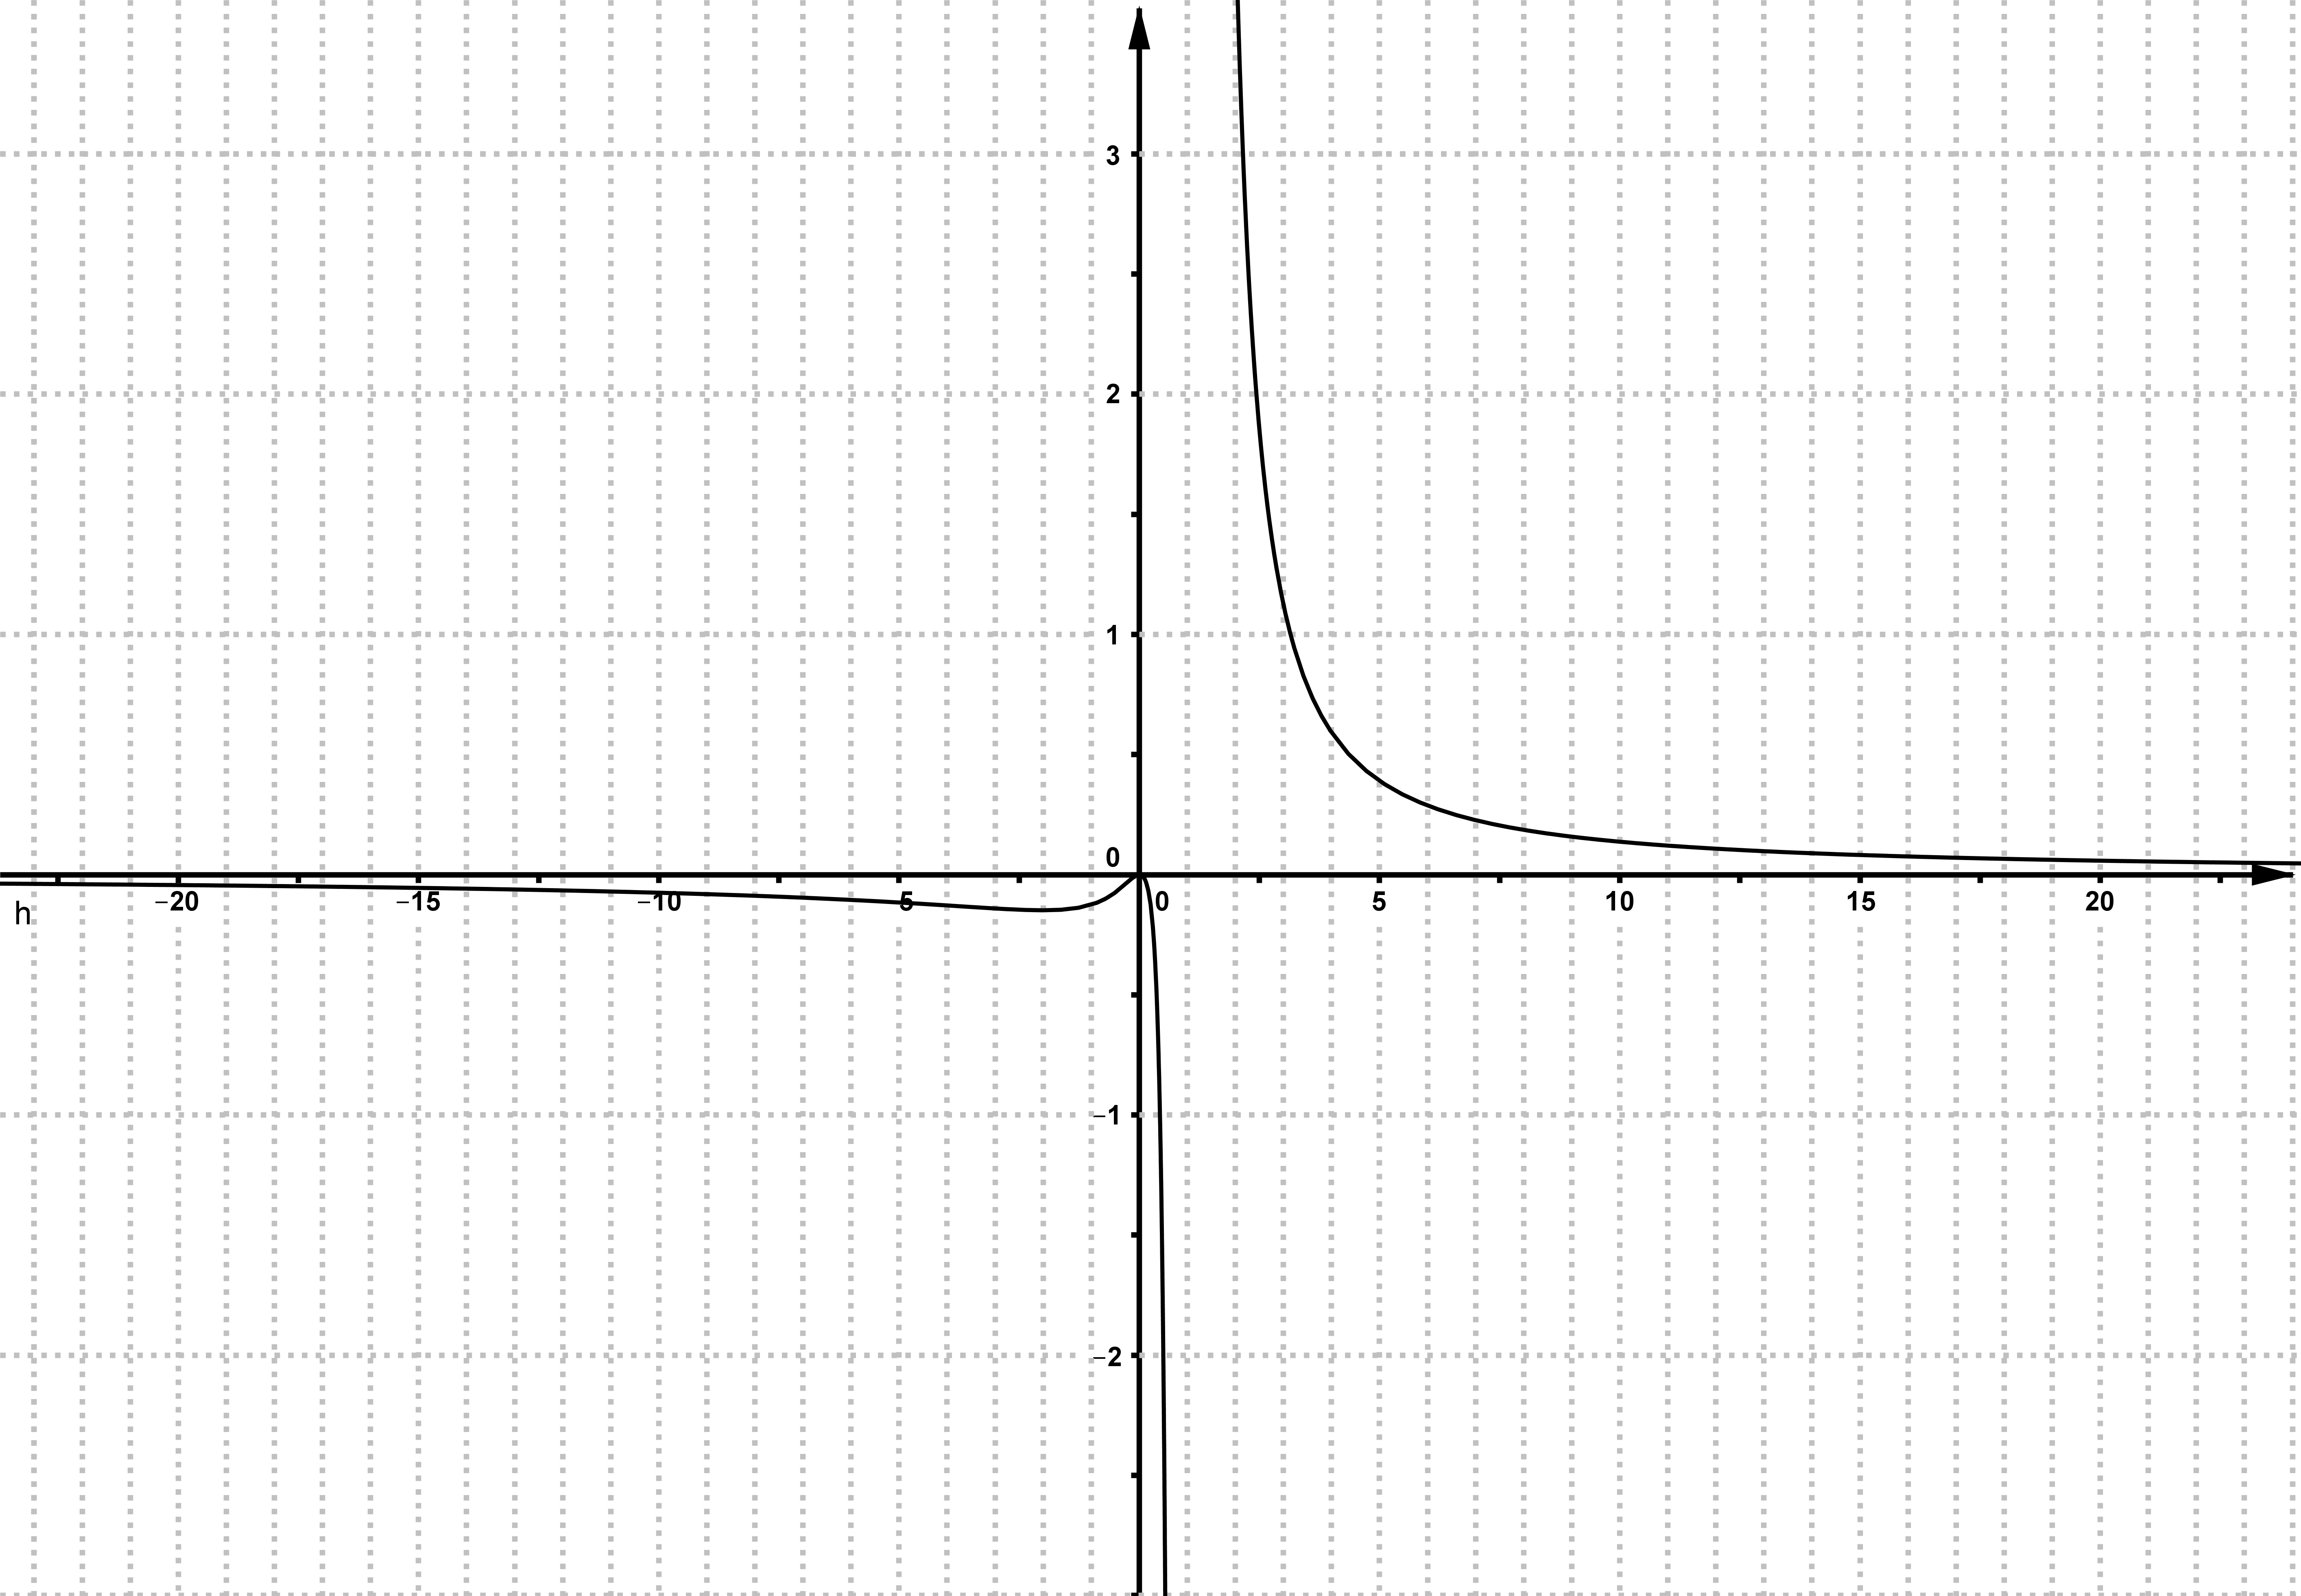
\includegraphics[width= 0.95\linewidth]{integradora3.png}
	%\end{figure}
	%graficos
\end{minipage}
\begin{minipage}{.5\textwidth}
	\centering
	%\begin{table}[!h]
	%\caption{mc1}
	%\label{mc1}
	\begin{tabular}{|c|c|c|}
		\hline
		$\frac{5x^2}{(x-2)(x+2)}$  & $\frac{x^2}{5(x-2)(x+2)}$ & $\frac{5(x-2)(x+2)}{x^3}$ \Ts \Bs   \\ \hline
		&   &      \\ \hline
	\end{tabular}\\
	%\end{table}
	%\begin{figure}[h]
	\centering
	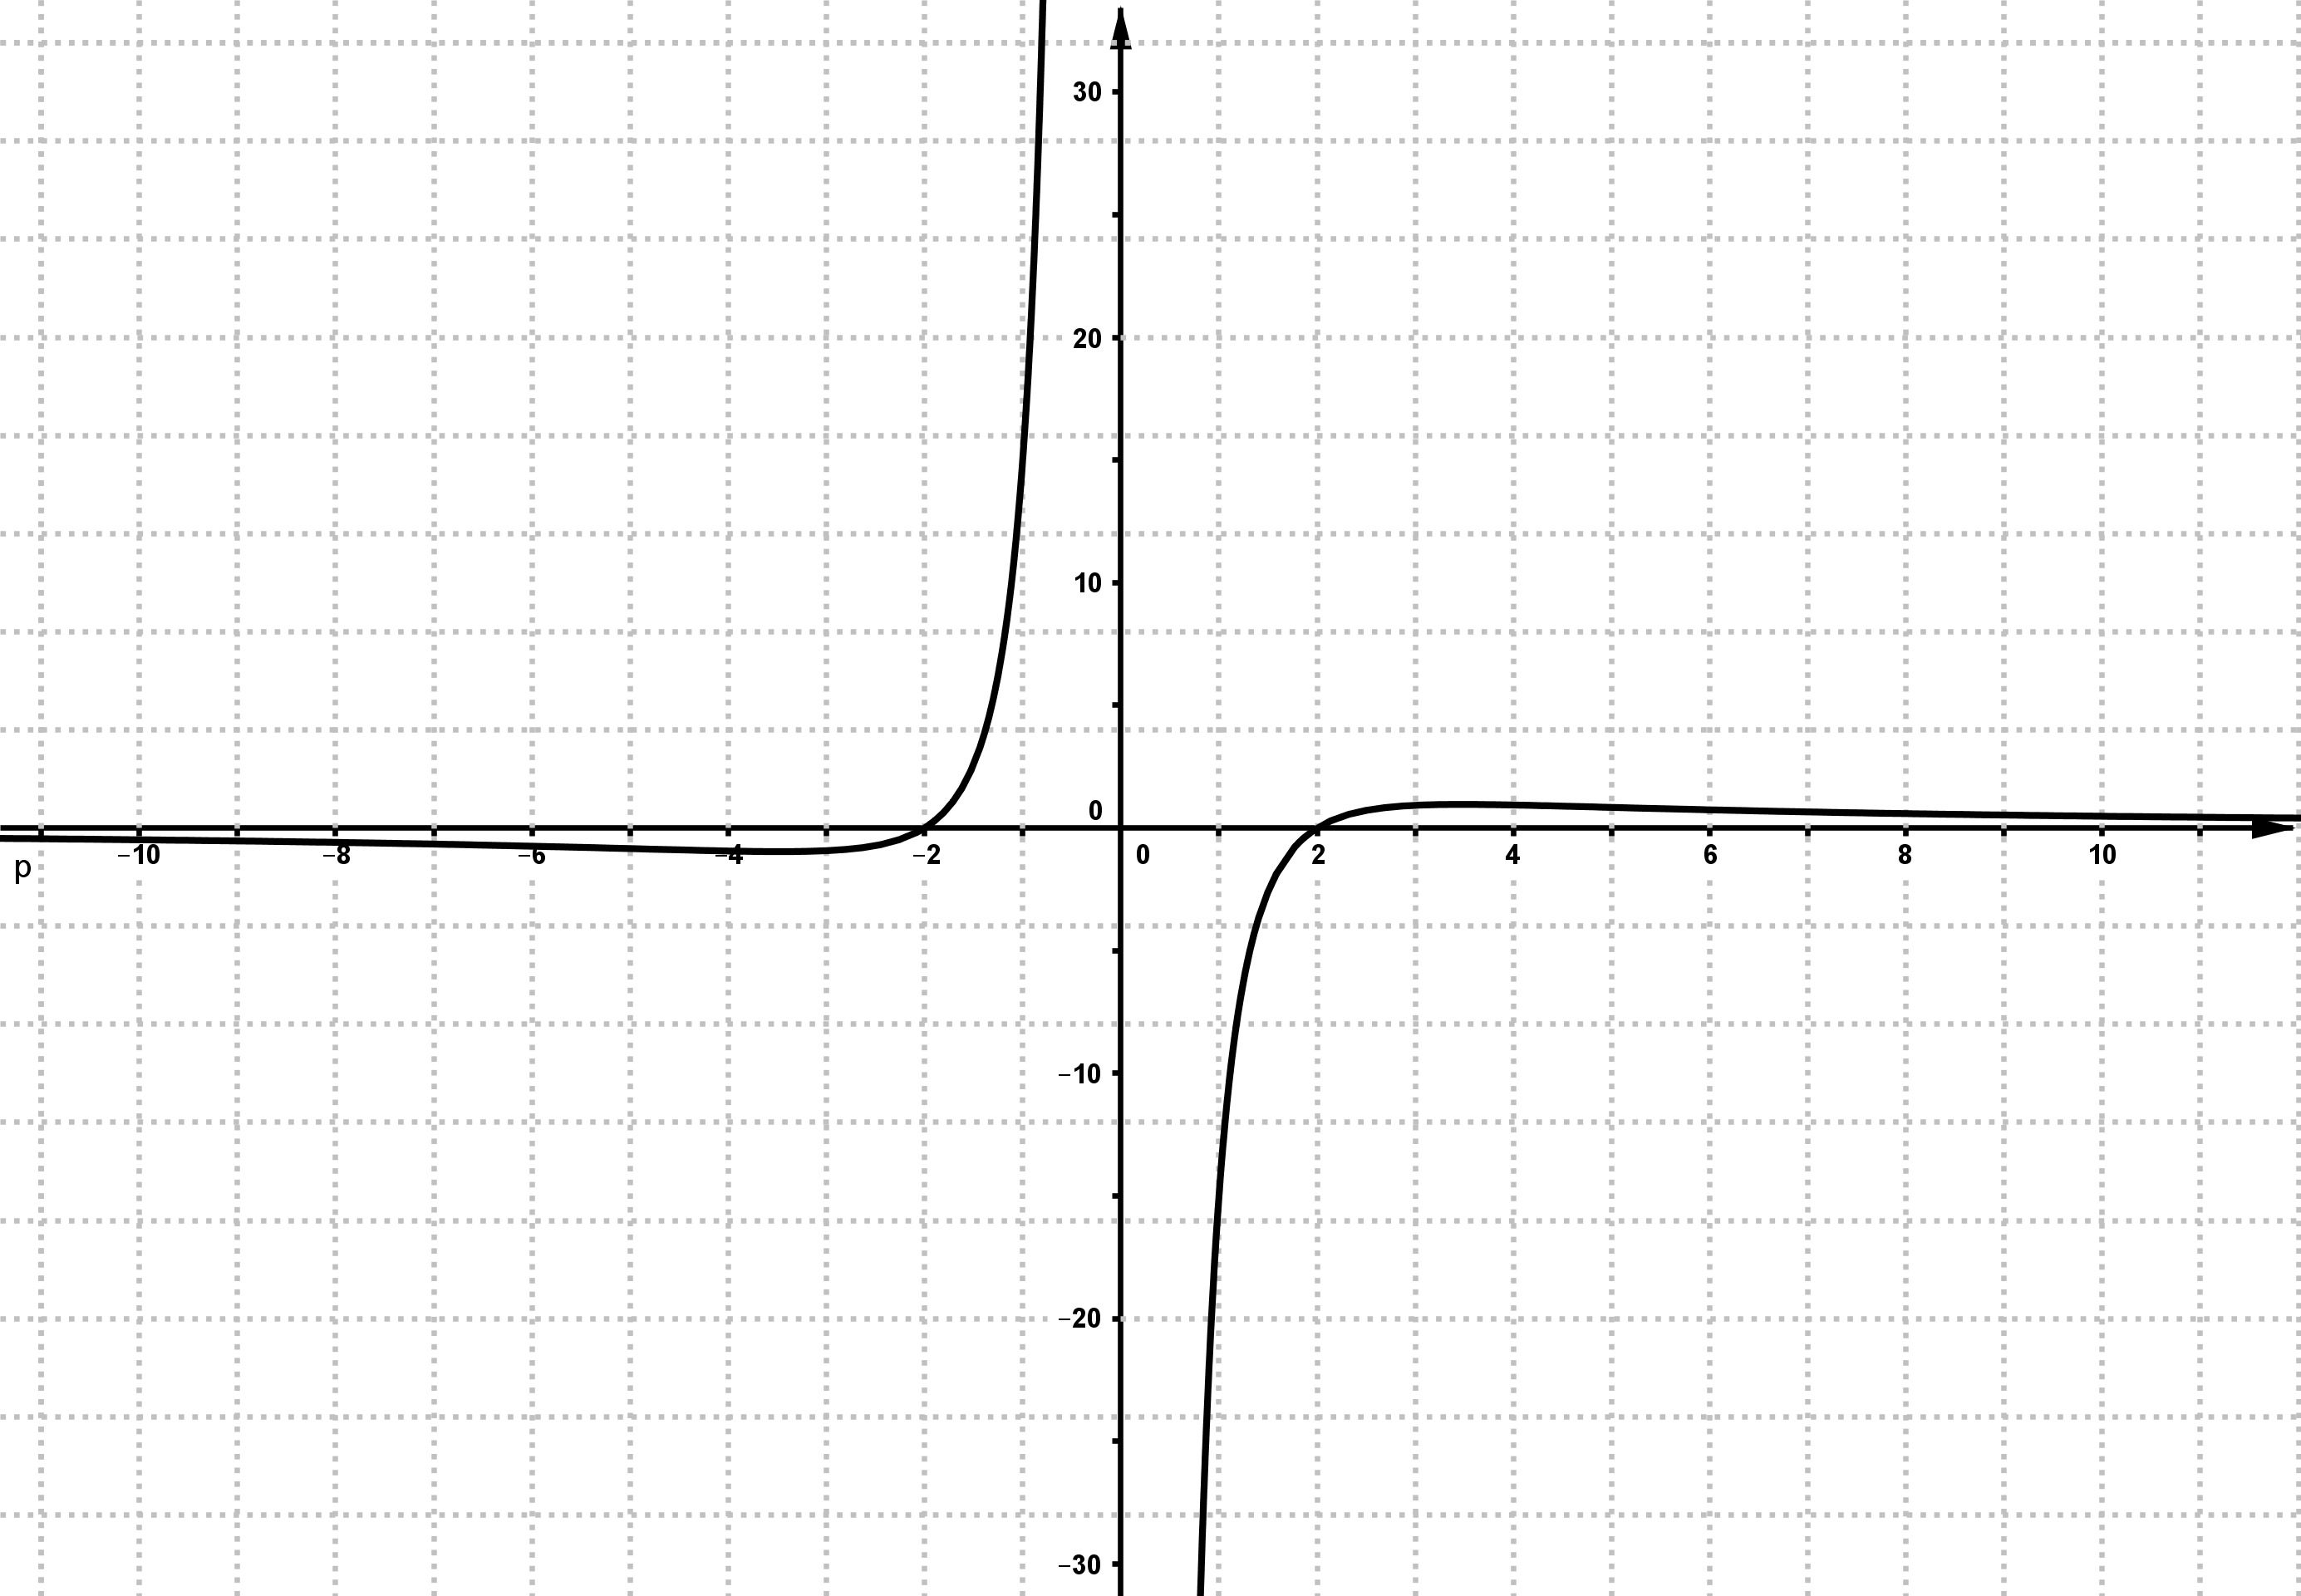
\includegraphics[width= 0.95\linewidth]{integradora4.png}
	%\end{figure}
\end{minipage}\\


2. Encontrar todos los valores de $x$ tal que: $\dfrac{3x-1}{x+1}>3$
\\

\section{Trigonometria (1,5 puntos)}
%\item Resolver los siguientes triángulos rectángulos. (Calcular los lados, los ángulos y sus razones trigonométricas). \label{rectangulos}\\

%	\begin{minipage}{0.45\linewidth}
%		
%		\begin{tikzpicture}[thick]
%		\coordinate (O) at (0,0);
%		\coordinate (A) at (3.5,0);
%		\coordinate (B) at (0,2.6);
%		\draw (O)--(A)--(B)--cycle;
%		
%		\tkzLabelSegment[below=2pt](O,A){$b$}
%		\tkzLabelSegment[left=2pt](O,B){$a$}
%		\tkzLabelSegment[above right=2pt](A,B){$h$}
%		
%		\tkzMarkRightAngle[fill=orange,size=0.6,opacity=.4](A,O,B)% square angle here
%		\tkzLabelAngle[pos = 0.35](A,O,B){$\hat{\gamma}$}
%		
%		\tkzMarkAngle[fill= orange,size=0.8cm,%
%		opacity=.4](B,A,O)
%		\tkzLabelAngle[pos = 0.6](B,A,O){$\hat{\alpha}$}
%		
%		\tkzMarkAngle[fill= orange,size=0.8cm,%
%		opacity=.4](O,B,A)
%		\tkzLabelAngle[pos = 0.5](O,B,A){$\hat{\beta}$}
%		
%		\end{tikzpicture}
%		
%	\end{minipage}
%	\begin{minipage}{0.55\linewidth}
%		\begin{enumerate}
%			%\item $a=3km$,  $\quad b=4km$ .	Expresar los resultados de los ángulos en el sistema sexagesimal.
%			%\item $a=2cm$, $\quad b=1cm$
%			\item $a=30km$,  $\quad b=20km$ .	Expresar los resultados de los ángulos en el sistema sexagesimal.
%			%\item $a=5cm$, $\quad \sin(\beta)=\frac{1}{\sqrt{2}}$. Expresar los resultados de los ángulos en Radianes.
%			%\item $a=5cm$, $\quad \cos(\alpha)=\frac{\sqrt{2}}{2}$
%			\item $a=5cm$, $\quad \cos(\alpha)=\frac{\sqrt{3}}{2}$ 
%		\end{enumerate}
%	\end{minipage}
Encontrar el lado restante y los ángulos internos.

\begin{tikzpicture}[thick]
\coordinate (O) at (0,0);
\coordinate (A) at (3,0);
\coordinate (B) at (2.5,1.5);
\draw (O)--(A)--(B)--cycle;

\tkzLabelSegment[below=2pt](O,A){$10m$}
\tkzLabelSegment[left=2pt](O,B){$15m$}
\tkzLabelSegment[above right=2pt](A,B){}

\tkzMarkAngle[fill=orange,size=0.3cm,opacity=.4](A,O,B)
\tkzLabelAngle[pos = -0.7](A,O,B){$\hat{\gamma}=30\degree $}

\tkzMarkAngle[fill= orange,size=0.3cm,%
opacity=.4](B,A,O)
\tkzLabelAngle[ pos= -0.4 ](B,A,O){$\hat{\alpha}$}

\tkzMarkAngle[fill= orange,size=0.3cm,%
opacity=.4](O,B,A)
\tkzLabelAngle[pos = -0.4](O,B,A){$\hat{\beta}$}
\end{tikzpicture}

\section{Complejos (1,5 puntos)}

\begin{enumerate}
	\item Resolver la siguiente ecuación, Graficar el resultado en el plano complejo.
	
	$(2x-5)i-4y+1=3-i$
\end{enumerate}


\textbf{\underline{Hoja de formulas}:} . \\

\begin{minipage}{0.5\linewidth}
	
	\begin{tikzpicture}[thick]
	\coordinate (O) at (0,0);
	\coordinate (A) at (3.5,0);
	\coordinate (B) at (-1,3);
	\draw (O)--(A)--(B)--cycle;
	
	\node at (O) [below left=2pt]{$a$};
	\node at (A) [right=2pt]{$b$};
	\node at (B) [above left=2pt]{$c$};
	
	\tkzLabelSegment[below=2pt](O,A){}
	\tkzLabelSegment[left=2pt](O,B){}
	\tkzLabelSegment[above right=2pt](A,B){}
	
	\tkzMarkAngle[fill=orange,size=0.6,opacity=.4](A,O,B)% square angle here
	\tkzLabelAngle[pos = 0.35](A,O,B){$\hat{a}$}
	
	\tkzMarkAngle[fill= orange,size=0.8cm,%
	opacity=.4](B,A,O)
	\tkzLabelAngle[pos = 0.6](B,A,O){$\hat{b}$}
	
	\tkzMarkAngle[fill= orange,size=0.7cm,%
	opacity=.4](O,B,A)
	\tkzLabelAngle[pos = 0.5](O,B,A){$\hat{c}$}
	\end{tikzpicture}
	
\end{minipage}
\begin{minipage}{0.5\linewidth}
	\textbf{Teorema del seno}:
	
	\[
	\frac{\overline{ab}}{\sin(\hat{c})}=\frac{\overline{ac}}{\sin(\hat{b})}=\frac{\overline{bc}}{\sin(\hat{a})}
	\]
	
	
	\textbf{Teorema del coseno}:
	
	\[
	\overline{ab}^2=\overline{ac}^2 + \overline{bc}^2 - 2.\overline{bc}.\overline{ac}.\cos(\hat{c})
	\]
\end{minipage}

Pitagoras: $
(cat.op)^2+(cat.ady)^2=h^2
$

Cuadráticas:

$y=ax^2+bx+c$

$y=a(x-x_v)^2+y_v$

$y=a(x-x_1)(x-x_2)$

$x_v=\frac{-b}{2a}$

Cambio de base: $\log_a(b)=\dfrac{\log_c(b)}{\log_c(a)}$

\rule[2ex]{\textwidth}{1pt}

“Eppur si muove” (y sin embargo se mueve..)  -Galileo Galilei 



\newpage

\noindent 
\begin{minipage}{0.92\linewidth}
	\begin{tabular*}{\textwidth}{l @{\extracolsep{\fill}} r @{\extracolsep{6pt}} l}
		\textbf{\class} & \textbf{Profesor: \examprof}\\
		\textbf{\examnumvulcano}  & \textbf{}   \\
		%& Teaching Assistant & %VII la venganza de adrian  \makebox[2in]{\hrulefill}
		\textbf{Nombre: } \makebox[2in]{\hrulefill} & \textbf{\examdate} 
	\end{tabular*}\\
\end{minipage}
\begin{minipage}[r]{0.08\linewidth}
	\begin{flushright}
		
\includegraphics[width=\linewidth]{bost.png}
	\end{flushright}
\end{minipage}\\
\rule[2ex]{\textwidth}{2pt}

\begin{center}
	\textsl{\textbf{\underline{Justificar}}} cada respuesta. La evaluación se entrega \textbf{\underline{escrita en tinta}}.\\
	Si se traban con un ejercicio sigan con el siguiente.
	May the force be with you.
\end{center}
\begin{table}[h]
	\centering
	%\caption{My caption}
	\label{my-label}
	\begin{tabular}{|l|c|c|c|c|c|c|c|c|c|}
		\hline
		Ejercicio        & 1 & 2 & 3 & 4 & 5 & 6 & 7 & Nota & Hojas \\ \hline
		Puntaje máximo   & 0,5 & 0,5 & 2 & 2 & 2 & 1,5 & 1,5 & 10 &  Entregadas \\ \hline
		Puntaje obtenido &   &   & & & & & &  &   \\ \hline
	\end{tabular}
\end{table}


\section{Numeros Reales y conjuntos (0,5 puntos) }
Graficar los conjuntos $\mathbb{N}$, $\mathbb{R}$, $\mathbb{Q}$, $\mathbb{C}$, $\mathbb{I}$, $\mathbb{Z}$, $\mathbb{I}m$ (imaginarios) como diagramas de Venn.

\section{Radicacion (0,5 puntos)}

\begin{enumerate}
	\item $\dfrac{\sqrt{7}-3}{3+\sqrt{7}}$
	\item $\dfrac{21}{3\sqrt{7}+7\sqrt{3}}$
\end{enumerate}

\section{Cuadraticas (2 puntos)}
\begin{enumerate}
	\item Bicuadratica: $x^4-8x^2+16=0$
	\item Graficar la siguiente función y expresarla en sus tres formas (normal, canónica y factorizada).
	
	$y=(x-1)^2-1 $
\end{enumerate}

\section{Logaritmos y exponenciales (2 puntos)}
\begin{enumerate}
	
	\item $2.\log_3(x)=4$
	
	\item Encontrar el valor de x para que $2^{x+1}-16=0$
	
\end{enumerate}


\section{Funciones Racionales (2 puntos)}

\begin{minipage}{0.5\textwidth}
	\centering
	%\begin{table}[!h]
	%\caption{mc1}
	\label{mc1}
	\begin{tabular}{|c|c|c|}
		\hline
		$\frac{x^2}{(x-1)^3}$  & $\frac{x^3}{(x-1)^2}$ & $\frac{x^3}{(x+1)^2}$ \Ts \Bs   \\ \hline
		&   &      \\ \hline
	\end{tabular}\\
	%\end{table}
	%\begin{figure}[h]
	\centering
	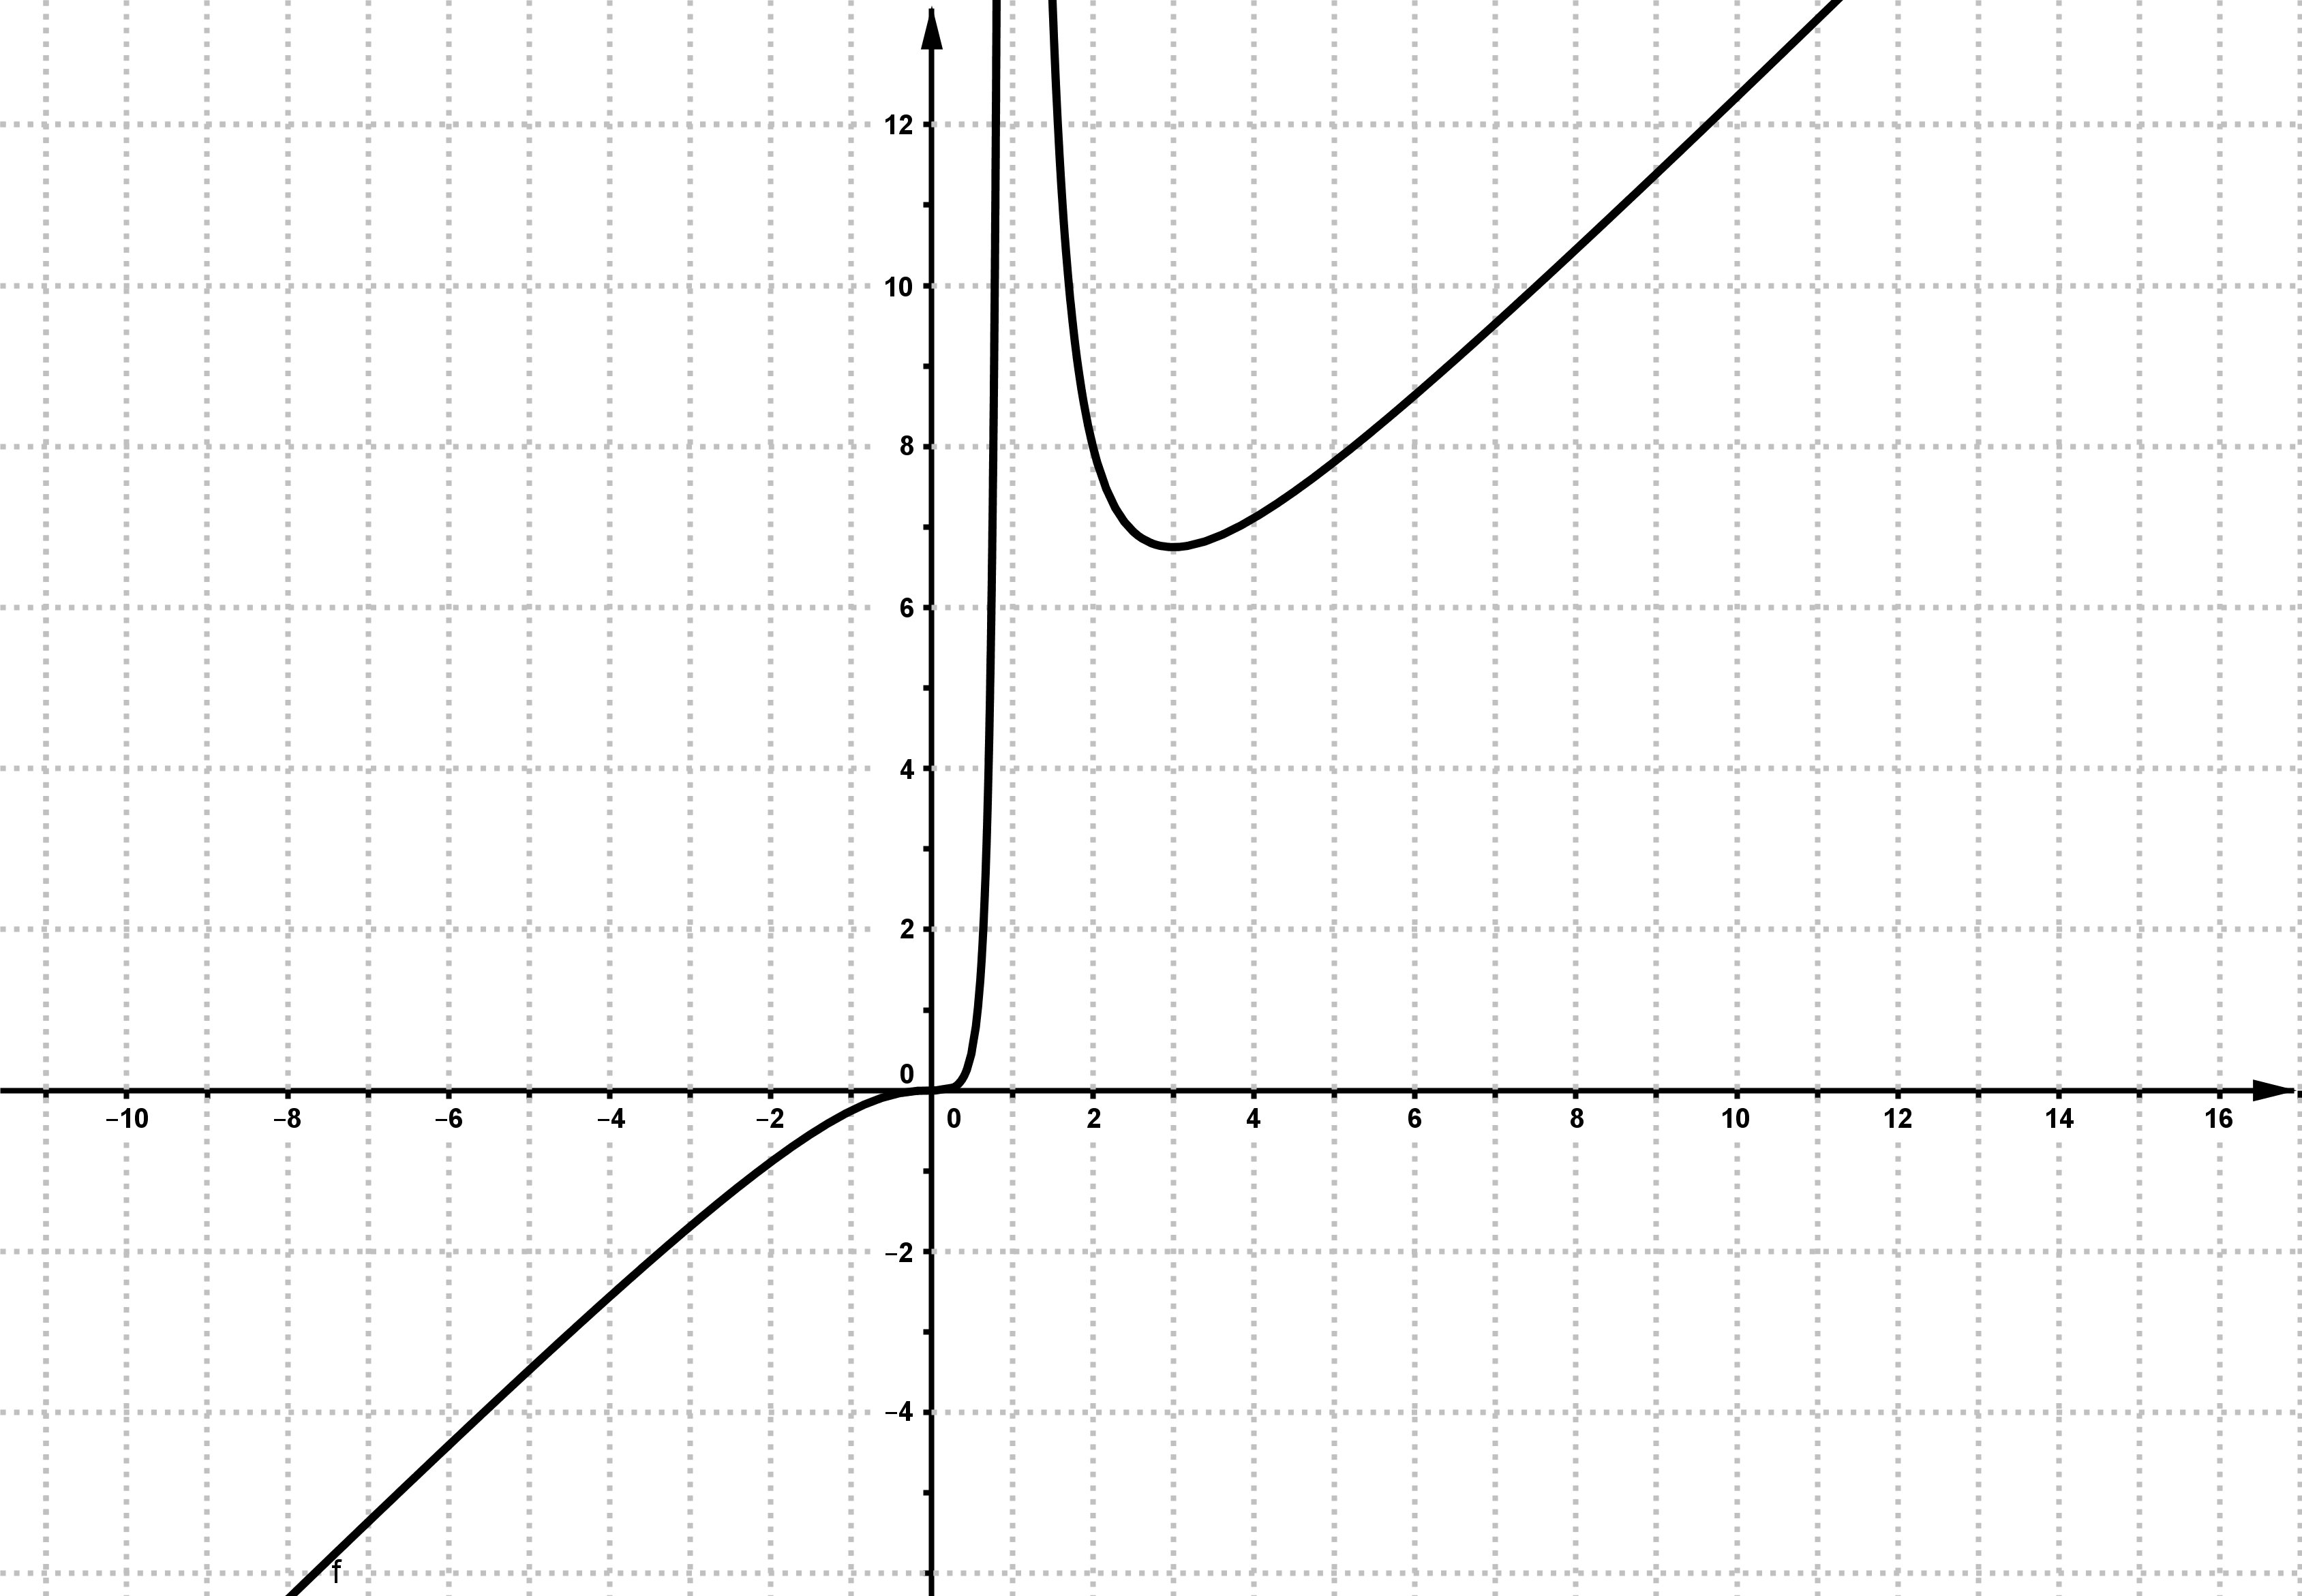
\includegraphics[width= 0.95\linewidth]{integradora1.png}
	%\end{figure}
	%graficos
\end{minipage}
\begin{minipage}{.5\textwidth}
	\centering
	%\begin{table}[!h]
	%\caption{mc1}
	%\label{mc1}
	\begin{tabular}{|c|c|c|}
		\hline
		$\frac{5x^2}{(x-2)(x+2)}$  & $\frac{x^2}{5(x-2)(x+2)}$ & $\frac{5(x-2)(x+2)}{x^3}$ \Ts \Bs   \\ \hline
		&   &      \\ \hline
	\end{tabular}\\
	%\end{table}
	%\begin{figure}[h]
	\centering
	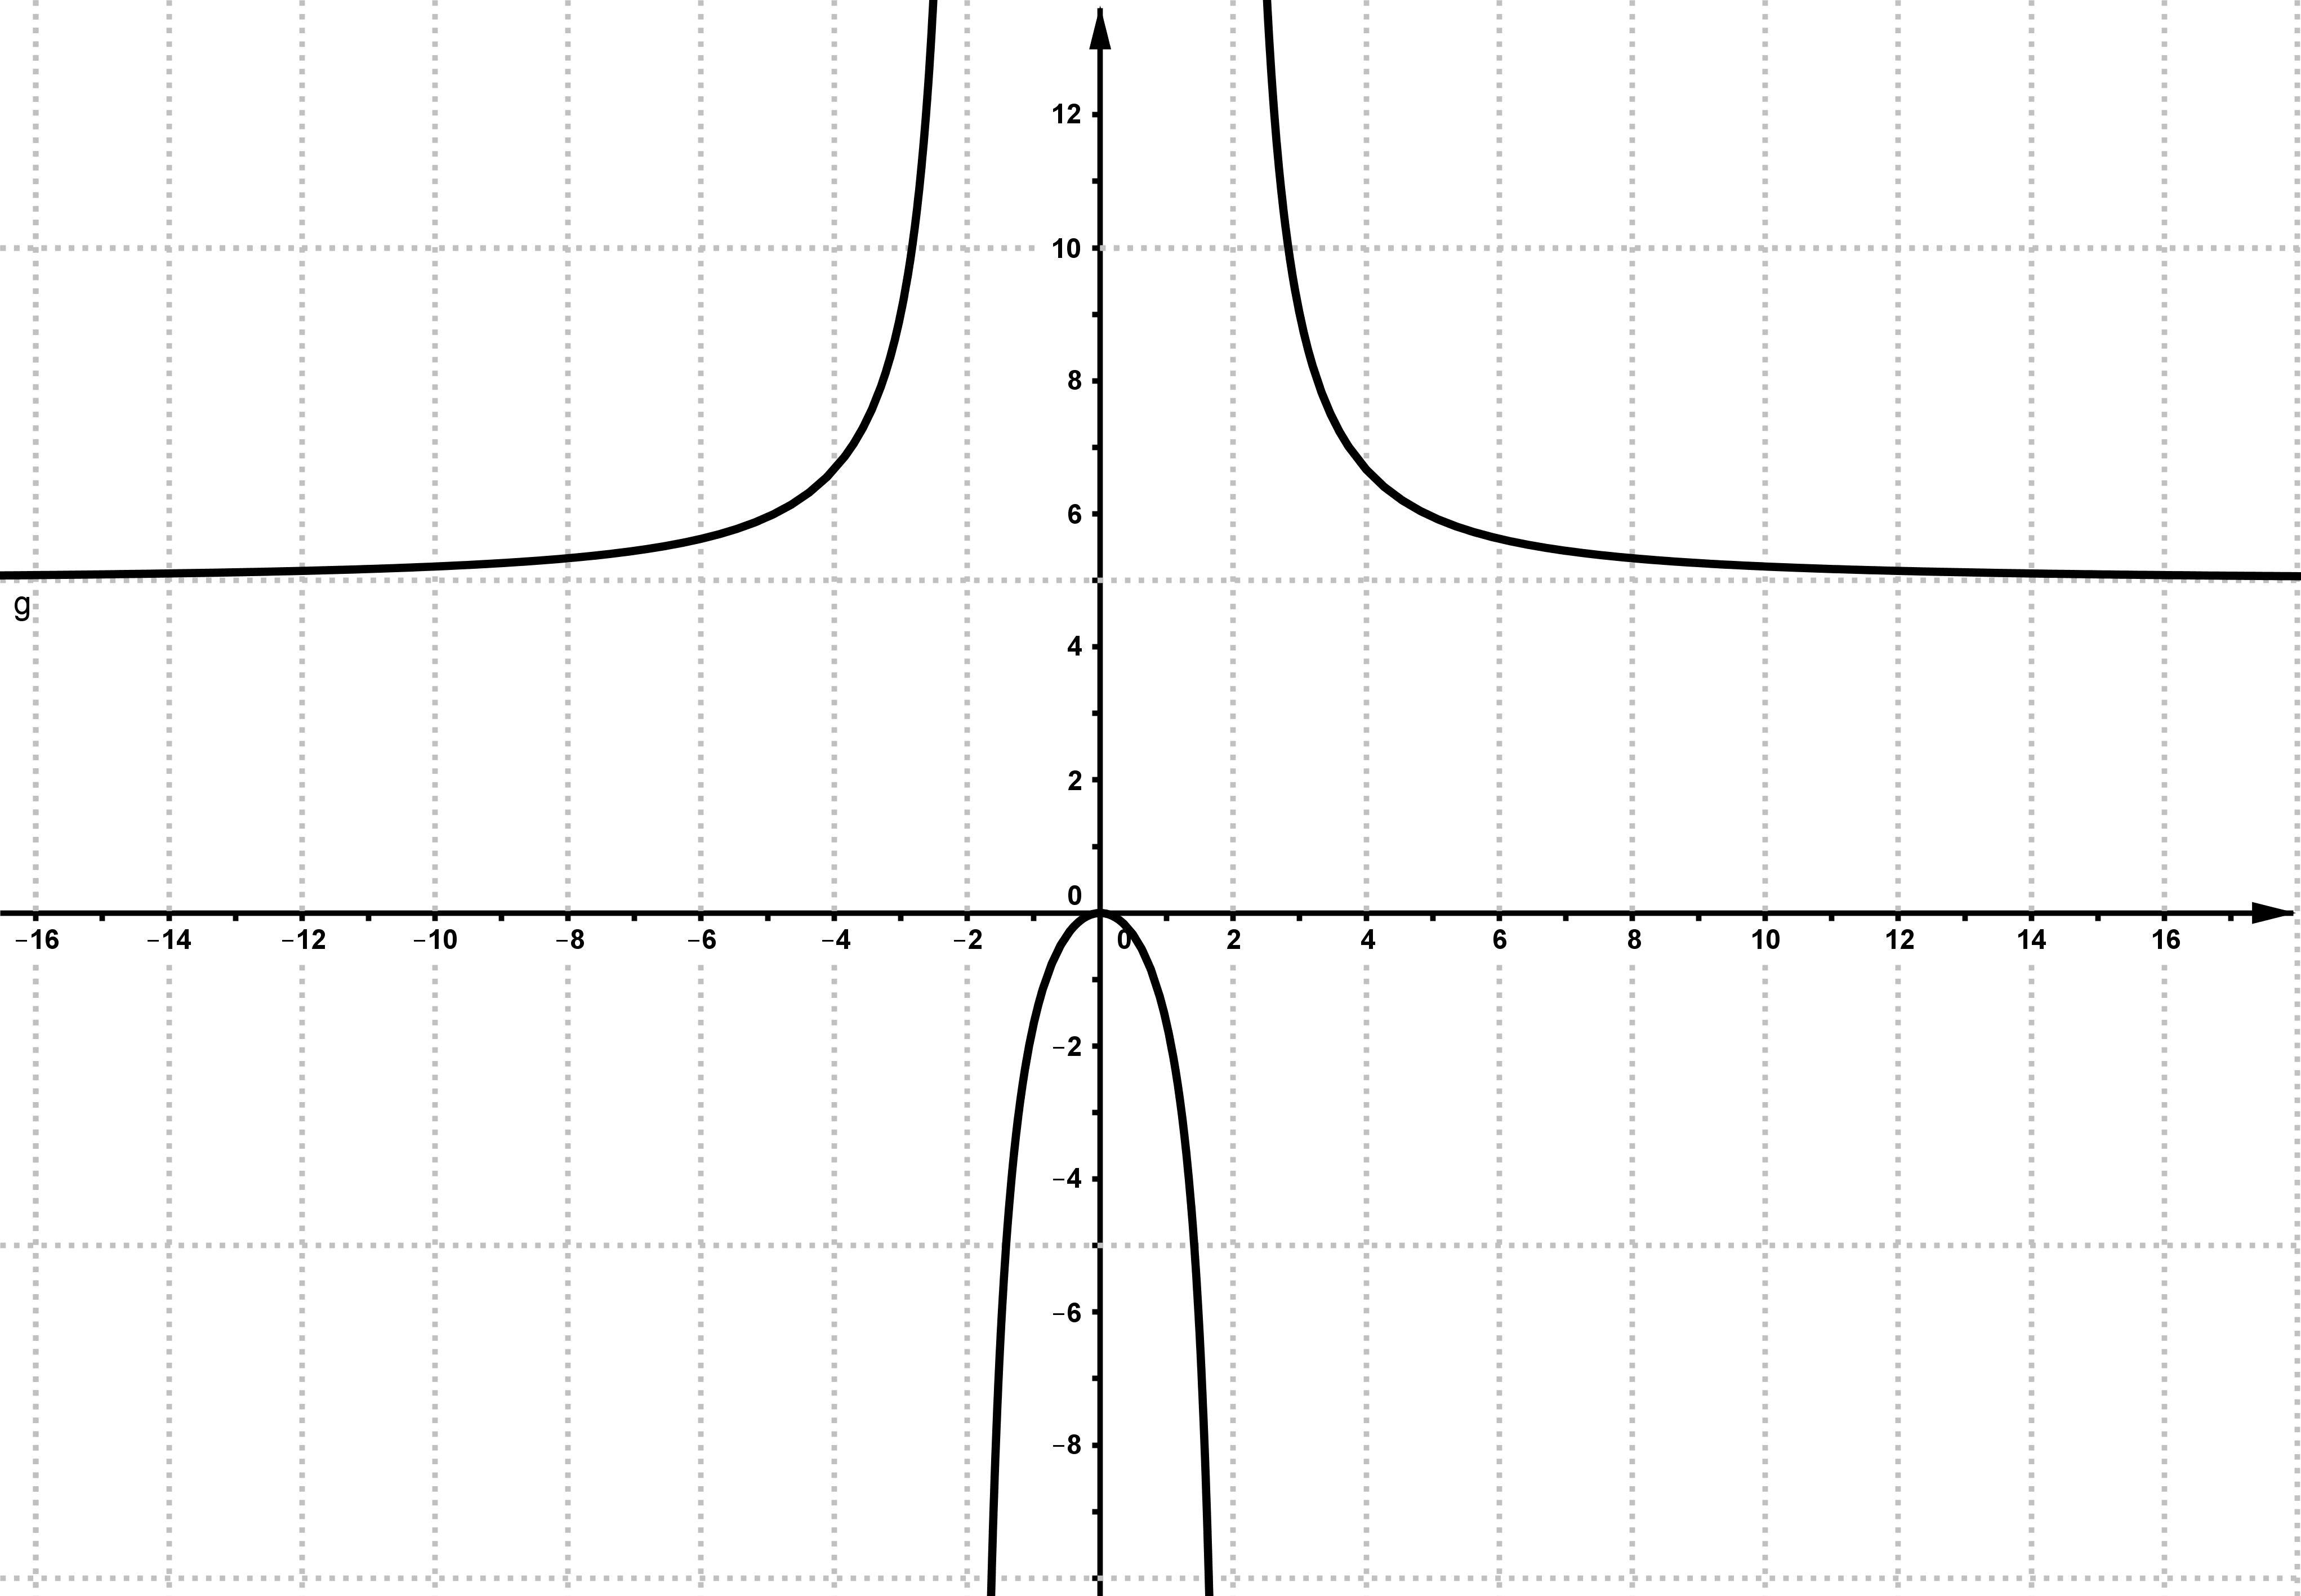
\includegraphics[width= 0.95\linewidth]{integradora2.png}
	%\end{figure}
\end{minipage}\\


2. Encontrar todos los valores de $x$ tal que: $\dfrac{3x-1}{x}>3$
\\

\section{Trigonometria (1,5 puntos)}
%\item Resolver los siguientes triángulos rectángulos. (Calcular los lados, los ángulos y sus razones trigonométricas). \label{rectangulos}\\

%	\begin{minipage}{0.45\linewidth}
%		
%		\begin{tikzpicture}[thick]
%		\coordinate (O) at (0,0);
%		\coordinate (A) at (3.5,0);
%		\coordinate (B) at (0,2.6);
%		\draw (O)--(A)--(B)--cycle;
%		
%		\tkzLabelSegment[below=2pt](O,A){$b$}
%		\tkzLabelSegment[left=2pt](O,B){$a$}
%		\tkzLabelSegment[above right=2pt](A,B){$h$}
%		
%		\tkzMarkRightAngle[fill=orange,size=0.6,opacity=.4](A,O,B)% square angle here
%		\tkzLabelAngle[pos = 0.35](A,O,B){$\hat{\gamma}$}
%		
%		\tkzMarkAngle[fill= orange,size=0.8cm,%
%		opacity=.4](B,A,O)
%		\tkzLabelAngle[pos = 0.6](B,A,O){$\hat{\alpha}$}
%		
%		\tkzMarkAngle[fill= orange,size=0.8cm,%
%		opacity=.4](O,B,A)
%		\tkzLabelAngle[pos = 0.5](O,B,A){$\hat{\beta}$}
%		
%		\end{tikzpicture}
%		
%	\end{minipage}
%	\begin{minipage}{0.55\linewidth}
%		\begin{enumerate}
%			%\item $a=3km$,  $\quad b=4km$ .	Expresar los resultados de los ángulos en el sistema sexagesimal.
%			%\item $a=2cm$, $\quad b=1cm$
%			\item $a=30km$,  $\quad b=20km$ .	Expresar los resultados de los ángulos en el sistema sexagesimal.
%			%\item $a=5cm$, $\quad \sin(\beta)=\frac{1}{\sqrt{2}}$. Expresar los resultados de los ángulos en Radianes.
%			%\item $a=5cm$, $\quad \cos(\alpha)=\frac{\sqrt{2}}{2}$
%			\item $a=5cm$, $\quad \cos(\alpha)=\frac{\sqrt{3}}{2}$ 
%		\end{enumerate}
%	\end{minipage}
Encontrar el lado restante y los ángulos internos.

\begin{tikzpicture}[thick]
\coordinate (O) at (0,0);
\coordinate (A) at (3,0);
\coordinate (B) at (2.5,1.5);
\draw (O)--(A)--(B)--cycle;

\tkzLabelSegment[below=2pt](O,A){$10m$}
\tkzLabelSegment[left=2pt](O,B){$15m$}
\tkzLabelSegment[above right=2pt](A,B){}

\tkzMarkAngle[fill=orange,size=0.3cm,opacity=.4](A,O,B)
\tkzLabelAngle[pos = -0.7](A,O,B){$\hat{\gamma}=30\degree $}

\tkzMarkAngle[fill= orange,size=0.3cm,%
opacity=.4](B,A,O)
\tkzLabelAngle[ pos= -0.4 ](B,A,O){$\hat{\alpha}$}

\tkzMarkAngle[fill= orange,size=0.3cm,%
opacity=.4](O,B,A)
\tkzLabelAngle[pos = -0.4](O,B,A){$\hat{\beta}$}
\end{tikzpicture}

\section{Complejos (1,5 puntos)}

\begin{enumerate}
	\item Resolver el siguiente problema y graficar el resultado en el plano complejo.
	
	$(i^2)\cdot((-2+i)+(i+4))$
\end{enumerate}


\textbf{\underline{Hoja de formulas}:} . \\

\begin{minipage}{0.5\linewidth}
	
	\begin{tikzpicture}[thick]
	\coordinate (O) at (0,0);
	\coordinate (A) at (3.5,0);
	\coordinate (B) at (-1,3);
	\draw (O)--(A)--(B)--cycle;
	
	\node at (O) [below left=2pt]{$a$};
	\node at (A) [right=2pt]{$b$};
	\node at (B) [above left=2pt]{$c$};
	
	\tkzLabelSegment[below=2pt](O,A){}
	\tkzLabelSegment[left=2pt](O,B){}
	\tkzLabelSegment[above right=2pt](A,B){}
	
	\tkzMarkAngle[fill=orange,size=0.6,opacity=.4](A,O,B)% square angle here
	\tkzLabelAngle[pos = 0.35](A,O,B){$\hat{a}$}
	
	\tkzMarkAngle[fill= orange,size=0.8cm,%
	opacity=.4](B,A,O)
	\tkzLabelAngle[pos = 0.6](B,A,O){$\hat{b}$}
	
	\tkzMarkAngle[fill= orange,size=0.7cm,%
	opacity=.4](O,B,A)
	\tkzLabelAngle[pos = 0.5](O,B,A){$\hat{c}$}
	\end{tikzpicture}
	
\end{minipage}
\begin{minipage}{0.5\linewidth}
	\textbf{Teorema del seno}:
	
	\[
	\frac{\overline{ab}}{\sin(\hat{c})}=\frac{\overline{ac}}{\sin(\hat{b})}=\frac{\overline{bc}}{\sin(\hat{a})}
	\]
	
	
	\textbf{Teorema del coseno}:
	
	\[
	\overline{ab}^2=\overline{ac}^2 + \overline{bc}^2 - 2.\overline{bc}.\overline{ac}.\cos(\hat{c})
	\]
\end{minipage}

Pitagoras: $
(cat.op)^2+(cat.ady)^2=h^2
$

Cuadráticas:

$y=ax^2+bx+c$

$y=a(x-x_v)^2+y_v$

$y=a(x-x_1)(x-x_2)$

$x_v=\frac{-b}{2a}$

Cambio de base: $\log_a(b)=\dfrac{\log_c(b)}{\log_c(a)}$

\rule[2ex]{\textwidth}{1pt}

“Eppur si muove” (y sin embargo se mueve..)  -Galileo Galilei 



\end{document}